\documentclass[12pt]{article}
\usepackage[margin=0.75in]{geometry}
\usepackage{graphicx}
\usepackage{float}
\setlength{\parindent}{0mm}

\begin{document}

{\centering
\large Physics 1111: Class 08 Activity \par
\large Work \par
}
\hfill \break \vspace{-4mm}

Consider using a constant horizontal force to push a block ($v_i = 0$) up a ramp that has friction.
Assume the coefficient of static friction is sufficiently small that the block immediately starts moving.
Use the following values: \\
$M = 3.0$ kg \\
$F = 26.0$ N \\
$\theta = 15^\circ$ \\
$\mu_k = 0.15$ \\
$t = 2.5$ s
%
\begin{figure}[H]
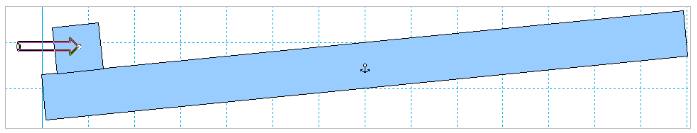
\includegraphics[scale=0.70]{fig.png}
\end{figure}
%
\begin{enumerate}
\item Draw a free body diagram for the block. For any force not parallel or perpendicular to the ramp, break it up into components.
\item Calculate the magnitude of each force, including components.
\item Use Newton's second law to calculate the acceleration of the block up the ramp.
\item Using the given time interval, calculate the final velocity, distance traveled, and final kinetic energy of the block.
\item Calculate the work done by each force.
\item Show that the total work done is equal to the change in kinetic energy.
\end{enumerate}

\end{document}
